\documentclass{article}
\usepackage{titlesec}
\usepackage[dotinlabels]{titletoc}
\usepackage[utf8]{inputenc}
\usepackage[russian]{babel}
\usepackage[a4paper, left=1.5cm, right=1.5cm, top=1cm, bottom=1cm]{geometry}
\usepackage[unicode, pdftex]{hyperref}
\setlength\parindent{0pt}
\pagenumbering{gobble}
\usepackage{caption} 
\captionsetup[table]{skip=5pt}
\usepackage{graphicx}
\usepackage{float}

\begin{document}

\begin{minipage}{0.62\textwidth}
    \begin{center}
        Санкт-Петербургский национальный исследовательский университет \\
        информационных технологий, механики и оптики \\
        УЧЕБНЫЙ ЦЕНТР ОБЩЕЙ ФИЗИКИ ФТФ
    \end{center}
\end{minipage}
\hfill
\begin{minipage}{0.38\textwidth}
    \centering
    \begin{figure}[H]
    
\includegraphics[width=\textwidth]{logo.png}
    \end{figure}
\end{minipage}

\rule{\textwidth}{1pt} \\

\begin{minipage}{0.16\textwidth}
        Группа \hrulefill\\
        Студент \hrulefill\\
        Преподаватель \hrulefill
\end{minipage}%
\begin{minipage}{0.25\textwidth}
        K3222\hrulefill\\
        Бевз Т.А.\hrulefill\\
        Соломонов А.И.\hrulefill
\end{minipage}
\hfill
\begin{minipage}{0.47\textwidth}
        К работе допущен \hrulefill\\
        Работа выполнена \hrulefill\\
        Отчёт принят \hrulefill
\end{minipage}
\begin{center}
    \textbf{\huge Рабочий протокол и отчет по \\
    лабораторной работе № 4.02}
\end{center}
\begin{minipage}{1\textwidth}
        \hrulefill\\
        \Large\textbf{Определение расстояния между щелями интерференционным методом}\hrulefill
\end{minipage}
\section{Цель работы}
\begin{enumerate}
     Определение расстояния между двумя щелями по полученной от них интерференционной картине.
\end{enumerate}

\section{Задачи, решаемые при выполнении работы}
\begin{enumerate}
    \item Измерение координат последовательных минимумов интерференционной картины.
    \item Расчет периода картины $\Delta x$.
    \item Построение графика зависимости ширины интерференционной полосы $\Delta x$ от расстояния между объектом и экраном $L$.
    \item Нахождение коэффициента наклона $K$ и его погрешности.
    \item Расчет расстояния между щелями $d$ и его погрешности.
\end{enumerate}

\section{Объект исследования}
Источник света, объект с щелями, экран, интерференционная картина.
\section{Метод экспериментального исследования}
Физический эксперимент.
\section{Рабочие формулы и исходные данные}
\begin{equation}
 \Delta x=\frac{\lambda}{d}\cdot L - \textit{Период интерференционной картины.}
 \label{eq:ref1}
\end{equation}
Где $\lambda$ - длина волны, $d$ - ширина щели, $L$ - расстояние от экрана
до объекта.
\begin{equation}
 d=\frac{\lambda}{K} - \textit{Расстояние между щелями.}
 \label{eq:ref2}
\end{equation}
Где $K$ - угловой коэффициент зависимости $\Delta x$ от $L$.
\begin{equation}
 \Delta_{z}=\sqrt{(\frac{\partial f}{\partial a}\Delta_{a})^2 + (\frac{\partial f}{\partial b}\Delta_{b})^2 + (\frac{\partial f}{\partial c}\Delta_{c})^2 + ...} - \textit{Погрешность искомой величины z как функции погрешностей прямо измеренных величин.}
 \label{eq:ref3}
\end{equation}
Где $\frac{\partial f}{\partial a}$; $\frac{\partial f}{\partial b}$; $\frac{\partial f}{\partial c}$; ... – частные производные искомой функции z
\newpage
\section{Измерительные приборы}
\begin{table}[h]
    \centering
    \bgroup
    \def\arraystretch{1.2}
    \begin{tabular}{|c|c|c|c|}
        \hline
        Наименоване & Тип прибора & Используемый диапазон & Погрешность \\
        \hline
        Оптический рельс & Аналоговый & $0-1200$ мм. & $0.5$ мм. \\
        \hline
        Миллиметровая шкала на экране & Аналоговый & $0-60$ мм. & $0.5$ мм. \\
        \hline
    \end{tabular}
    \egroup
    \caption{Измерительные приборы} 
\end{table}
\section{Схема установки}
\begin{figure}[h!]
    \begin{center}
    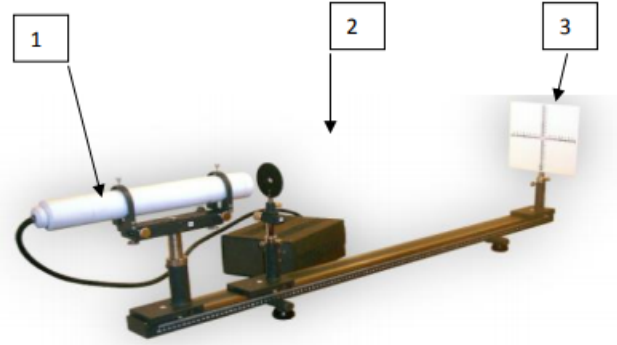
\includegraphics[width=0.6\textwidth]{scheme.png}
    \caption{Фото экспериментальной установки. 1 – лазер, 2 – объект, 3 – экран.}
    \label{fig:scheme}    
    \end{center}
\end{figure}
\section{Ход работы}
\begin{itemize}
  \item Для обработки результатов лабораторной работы было необходимо измерить координаты десяти последовательных минимумов интерференционных картин при различных положениях объекта. Результаты измерений представлены в таблице №2. Где $x_{0}$ - координата положения объекта, а $x_{1}...x_{10}$ - координаты последовательных минимумов картин, при определенном положении объекта.
  \item Далее для каждого измерения было вычислено расстояние между объектом и экраном $L$ и значение периода картины $\Delta x$. Координата экрана $X_{\textbf{э}}=1200$ мм. Вычисления представлены в таблице №3.
  \item На основе полученных данных был построен и апроксимирован график зависимости $ \Delta x(L) $. График представлен на рисунке №2.
  \item После этого, при помощи метода наименьших квадратов был найден коэффициент $K = 0.00395$ и его погрешность, которая составила $ \Delta K = 0.00023 $.
  \item Наконец, по известной длине волны $\lambda$ и коэффициенту $ K $ было рассчитано расстояние между щелями $d = 0.16$ мм. Также с помощью рекомендаций из пособия по обработке экспериментальных данных была определена его погрешность $\Delta d = 0.009$ мм.
\end{itemize}
\section{Результаты прямых измерений и их обработки}
\begin{table}[h]
    \centering
    \bgroup
    \def\arraystretch{1.4}
    \begin{tabular}{|c|c|c|c|c|c|c|c|c|c|c|c|}
        \hline
        № & $x_{0}$, мм & $x_{1}$, мм & $x_{2}$, мм & $x_{3}$, мм & $x_{4}$, мм & $x_{5}$, мм & $x_{6}$, мм & $x_{7}$, мм & $x_{8}$, мм & $x_{9}$, мм & $x_{10}$, мм \\ \hline
        $ 1 $ & $ 160 $ & $ 4 $ & $ 8 $ & $ 13 $ & $ 18 $ & $ 22 $ & $ 26 $ & $ 32 $ & $ 37 $ & $ 41 $ & $ 46 $\\ \hline
        $ 2 $ & $ 230 $ & $ 4 $ & $ 8 $ & $ 12 $ & $ 17 $ & $ 21 $ & $ 24 $ & $ 30 $ & $ 34 $ & $ 39 $ & $ 43 $\\ \hline
        $ 3 $ & $ 300 $ & $ 3 $ & $ 7 $ & $ 11 $ & $ 16 $ & $ 19 $ & $ 22 $ & $ 28 $ & $ 31 $ & $ 35 $ & $ 39 $\\ \hline
        $ 4 $ & $ 370 $ & $ 3 $ & $ 7 $ & $ 11 $ & $ 15 $ & $ 18 $ & $ 22 $ & $ 26 $ & $ 30 $ & $ 33 $ & $ 37 $\\ \hline
        $ 5 $ & $ 450 $ & $ 3 $ & $ 7 $ & $ 10 $ & $ 13 $ & $ 17 $ & $ 20 $ & $ 24 $ & $ 27 $ & $ 30 $ & $ 33 $\\ \hline
        $ 6 $ & $ 540 $ & $ 3 $ & $ 6 $ & $ 9 $ & $ 12 $ & $ 15 $ & $ 18 $ & $ 21 $ & $ 24 $ & $ 27 $ & $ 30 $\\ \hline
    \end{tabular}
    \egroup
    \caption{Координаты последовательных минимумов.} 
\end{table}
\begin{table}[h]
    \centering
    \bgroup
    \def\arraystretch{1.4}
    \begin{tabular}{|c|c|c|c|c|}
        \hline
        № & $X_{0}$, мм & $L$, мм & $x_{10}-x_{1}$, мм & $\Delta x$, мм\\ \hline
        $1$ & $ 160 $ & $ 1040 $ & $ 42 $ & $ 4.2 $\\ \hline
        $2$ & $ 230 $ & $ 970 $ & $ 39 $ & $ 3.9 $\\ \hline
        $3$ & $ 300 $ & $ 900 $ & $ 36 $ & $ 3.6 $\\ \hline
        $4$ & $ 370 $ & $ 830 $ & $ 34 $ & $ 3.4 $\\ \hline
        $5$ & $ 450 $ & $ 750 $ & $ 30 $ & $ 3 $\\ \hline
        $6$ & $ 540 $ & $ 660 $ & $ 27 $ & $ 2.7 $\\ \hline
    \end{tabular}
    \egroup
    \caption{Периоды интерференционных полос.} 
\end{table}
\newpage
\section{Графики}
\begin{figure}[h!]
    \begin{center}
    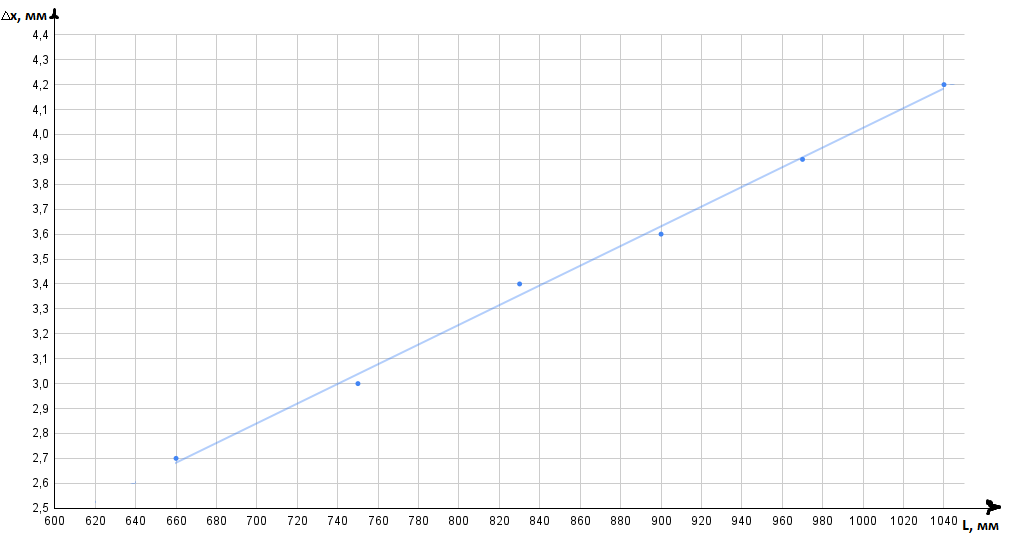
\includegraphics[scale=0.7]{chart.png}
    \caption{Зависимость $\Delta x$ от $L$}
    \label{fig:graphUfromI}    
    \end{center}
\end{figure}
\newpage
\section{Окончательные результаты}
\begin{enumerate}
    \item Коэффициент наклона: $K = (39.5 \pm 2.3 )\cdot 10^{-4}$; $\varepsilon_{K} = 6\%$  
    \item Расстояние между щелями: $d = (160 \pm 9 )$ мкм; $\varepsilon_{d} = 6\%$  
\end{enumerate}
\newpage
\section{Вывод}
Входе работы была исследована интерференционная картина от двух щелей методом Юнга. Были получены значения периода картины и построен график его зависимости от расстояния между объектом и экраном, благодаря этим значениям был найден коэффициент наклона. Было найдено расстояние между щелями, по полученной от них интерференционной картины.
\end{document}
